\documentclass{article}
\usepackage[utf8]{inputenc}
\usepackage[T1]{fontenc}
\usepackage{tikz}
\usepackage{amssymb} % Required for \square symbol

% TikZ libraries for the diagram
\usetikzlibrary{automata, positioning, arrows}

% Defining the blank symbol command
\newcommand{\blank}{\square}

\begin{document}

\begin{center}
\textbf{\Large Decider TM for $L = \{ a^n b^n \mid n \geq 0 \}$}\\[0.3cm]
\end{center}

% ==========================================
% PART 1: TAPE
% ==========================================
\begin{center}
\textbf{Execution Example (Initial Tape)}
\vspace{0.5cm}

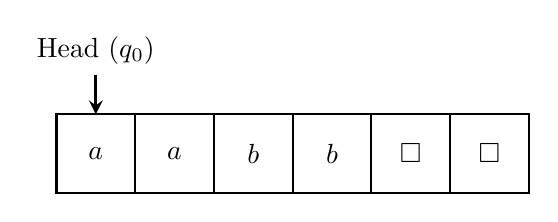
\begin{tikzpicture}[thick]
  % Drawing the tape: a, a, b, b, blank, blank
  \foreach \sym [count=\i] in {a, a, b, b, \blank, \blank} {
    \draw (\i-1, 0) rectangle +(1, 1);
    \node at (\i-0.5, 0.5) {$\sym$};
  }
  
  % Drawing the read head at position 1 (q0 reading 'a')
  \draw[->, >=stealth, very thick] (0.5, 1.5) -- (0.5, 1.0);
  \node[above] at (0.5, 1.5) {Head ($q_0$)};
\end{tikzpicture}
\end{center}

\hrule

% ==========================================
% PART 2: STATE DIAGRAM (Logic)
% ==========================================
\begin{center}
\textbf{State Diagram}
\vspace{0.5cm}

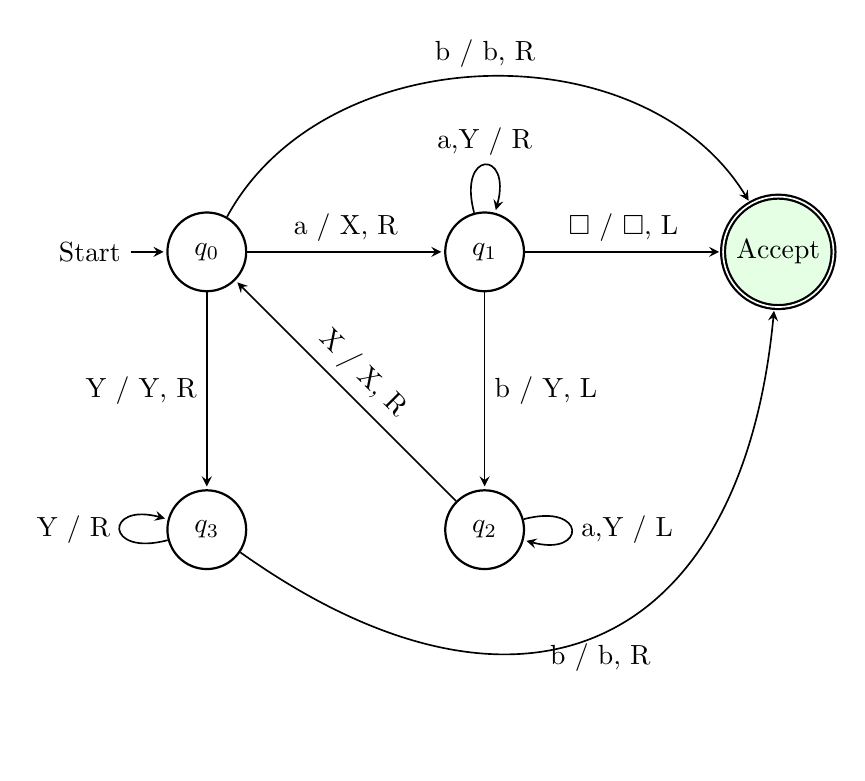
\begin{tikzpicture}[
    ->,
    >=stealth,
    shorten >=1pt,
    auto,
    node distance=2.5cm, % Increased distance for spacing
    semithick,
    state/.style={circle, draw, minimum size=10mm, thick, fill=white},
    accept/.style={double, circle, draw, minimum size=10mm, thick, fill=green!10}
  ]

  % --- STATE DEFINITIONS ---
  \node[state, initial, initial text=Start] (q0) {$q_0$};
  \node[state, right=of q0] (q1) {$q_1$};
  \node[state, below=of q0] (q3) {$q_3$};
  \node[state, below=of q1] (q2) {$q_2$};
  \node[accept, right=of q1] (acc) {Accept};

  % --- TRANSITIONS ---
  
  % From q0
  \path (q0) edge node {a / X, R} (q1)
             % Increased bend left to 60 to pass well above q1
             edge[bend left=60] node {b / b, R} (acc) 
             edge node[left] {Y / Y, R} (q3);

  % From q1
  \path (q1) edge[loop above] node {a,Y / R} (q1)
             edge node {$\blank$ / $\blank$, L} (acc)
             edge node[right] {b / Y, L} (q2);

  % From q2
  \path (q2) edge[loop right] node {a,Y / L} (q2)
             edge node[above, sloped] {X / X, R} (q0);

  % From q3
  \path (q3) edge[loop left] node {Y / R} (q3)
             % bend right=100 creates a large curve below
             % looseness=1.5 makes the curve more "open" to avoid hitting q2
             edge[bend right=60, looseness=1.5] node[below] {b / b, R} (acc);

\end{tikzpicture}

% --- LEGEND ---
\noindent
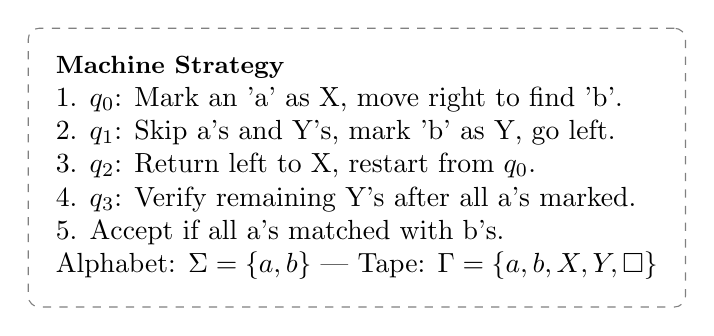
\begin{tikzpicture}
\node[draw=black!50, dashed, rounded corners, inner sep=10pt, align=left] {
  \small
  \textbf{Machine Strategy}\\
  1. $q_0$: Mark an 'a' as X, move right to find 'b'.\\
  2. $q_1$: Skip a's and Y's, mark 'b' as Y, go left.\\
  3. $q_2$: Return left to X, restart from $q_0$.\\
  4. $q_3$: Verify remaining Y's after all a's marked.\\
  5. Accept if all a's matched with b's.\\
  Alphabet: $\Sigma = \{a, b\}$ | Tape: $\Gamma = \{a, b, X, Y, \blank\}$
};
\end{tikzpicture}

\end{center}

\end{document}
